%
%===============>>  ГРУППА 11-1 МОДУЛЬ 4  <<=============
%
\setmodule{4}
%
%===============>>  Занятие 1  <<===============
%
%\begin{class}[number=1]
%	\begin{listofex}
%		\item Пусто
%	\end{listofex}
%\end{class}
%
%===============>>  Занятие 2  <<===============
%
%\begin{class}[number=2]
%	\begin{listofex}
%		\item Пусто
%	\end{listofex}
%\end{class}
%
%===============>>  Домашняя работа 1  <<===============
%
%\begin{homework}[number=1]
%	\begin{listofex}
%		\item Пусто
%	\end{listofex}
%\end{homework}
%
%===============>>  Занятие 3  <<===============
%
%\begin{class}[number=3]
%	\begin{listofex}
%		\item Пусто
%	\end{listofex}
%\end{class}
%
%===============>>  Занятие 4  <<===============
% смещение на одно занятие с прошлого месяца
%\begin{class}[number=4]
%	\begin{listofex}
%		\item Пусто
%	\end{listofex}
%\end{class}
%
%===============>>  Домашняя работа 2  <<===============
%
\begin{homework}[number=2]
	\begin{listofex}
		\item
	\end{listofex}
\end{homework}
%
%===============>>  Занятие 5  <<===============
% смещение на одно занятие с прошлого месяца
\begin{class}[number=5]
	\begin{listofex}
		\item
		\begin{minipage}[t]{0.43\textwidth}
			На рисунке изображён график функции вида \(f(x)=\dfrac{k}{x}+a\). Найдите, при каком значение \( x \) значение функции равно \(0,8\).
		\end{minipage}
		\begin{minipage}[c]{0.1\textwidth}
			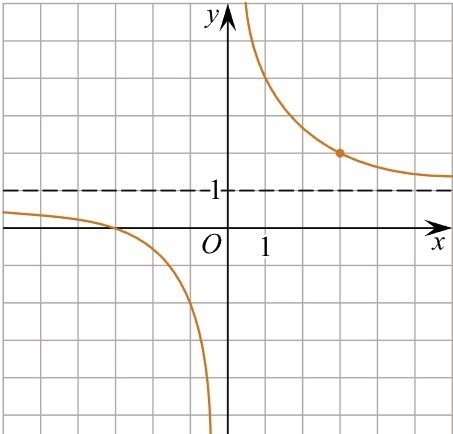
\includegraphics[align=t, width=\textwidth]{pics/G101M4C5-1.jpg}
		\end{minipage}
		\item
		\begin{minipage}[t]{0.43\textwidth}
			На рисунке изображён график функции вида \(f(x)=\dfrac{a}{x+b}+c\), где числа \(a, b, c\) --- целые. Найдите \(f(4)\).
		\end{minipage}
		\begin{minipage}[c]{0.1\textwidth}
			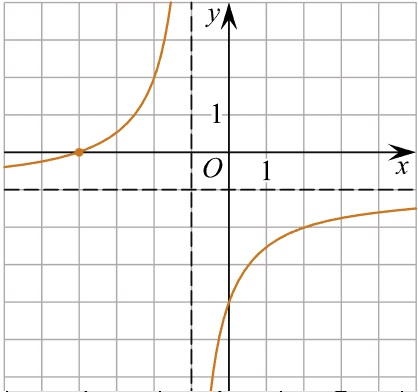
\includegraphics[align=t, width=\textwidth]{pics/G101M4C5-3.jpg}
		\end{minipage}
		\item
		\begin{minipage}[t]{0.43\textwidth}
			На рисунке изображён график функции вида \(f(x)=\dfrac{ax+b}{x+c}\), где числа \(a, b, c\) --- целые. Найдите \(a\).
		\end{minipage}
		\begin{minipage}[c]{0.1\textwidth}
			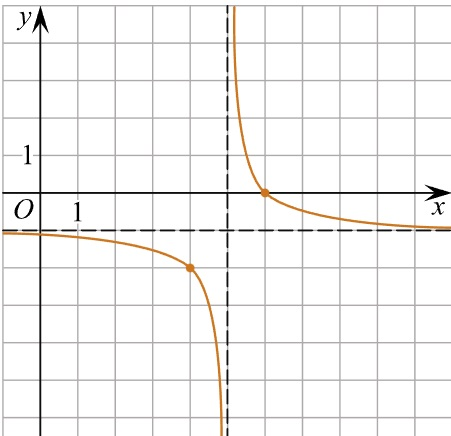
\includegraphics[align=t, width=\textwidth]{pics/G101M4C5-5.jpg}
		\end{minipage}
		\item
		\begin{minipage}[t]{0.43\textwidth}
			На рисунке изображён график функции вида \(f(x)=\dfrac{a}{x+b}+c\), где числа \(a, b, c\) --- целые. Найдите \(f\left(\dfrac{1}{3}\right)\).
		\end{minipage}
		\begin{minipage}[c]{0.1\textwidth}
			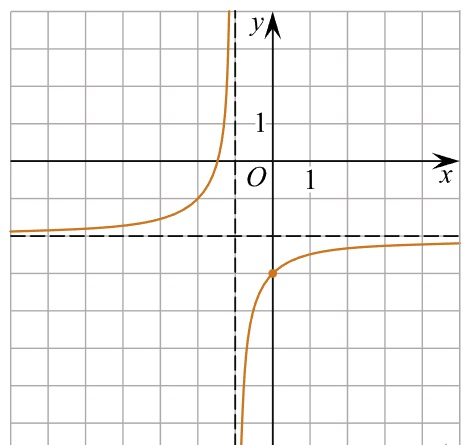
\includegraphics[align=t, width=\textwidth]{pics/G111M4C5-1.jpg}
		\end{minipage}
		\item
		\begin{minipage}[t]{0.43\textwidth}
			На рисунке изображён график функции вида \(f(x)=\dfrac{a}{x+b}+c\), где числа \(a, b, c\) --- целые. Найдите \(-3\).
		\end{minipage}
		\begin{minipage}[c]{0.1\textwidth}
			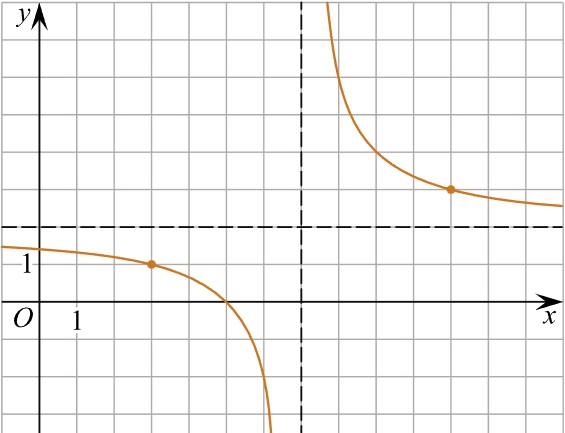
\includegraphics[align=t, width=\textwidth]{pics/G111M4C5-2.jpg}
		\end{minipage}
		\item
		\begin{minipage}[t]{0.43\textwidth}
			На рисунке изображён график функции вида \(f(x)=ax-|bx+c|+d\), где числа \(a, b, c, d\) --- целые. Найдите корень уравнения \(ax+d=0\).
		\end{minipage}
		\begin{minipage}[c]{0.11\textwidth}
			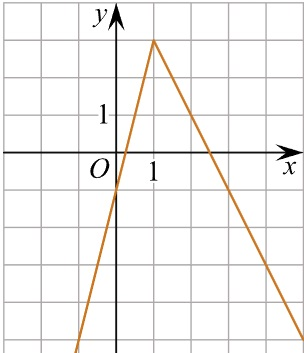
\includegraphics[align=t, width=\textwidth]{pics/G111M4C5-3.jpg}
		\end{minipage}
		\item
		\begin{minipage}[t]{0.43\textwidth}
			На рисунке изображён график функции вида \(f(x)=ax+|bx+c|+d\), где числа \(a, b, c, d\) --- целые. Найдите корень уравнения \(ax+d=10\).
		\end{minipage}
		\begin{minipage}[c]{0.1\textwidth}
			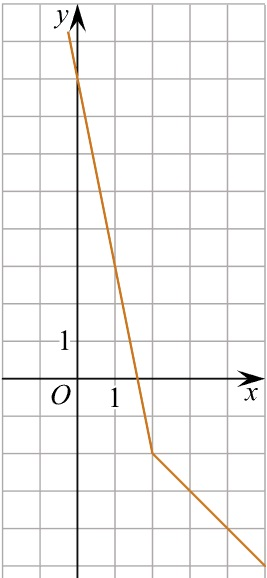
\includegraphics[align=t, width=\textwidth]{pics/G111M4C5-4.jpg}
		\end{minipage}
		\item
		\begin{minipage}[t]{0.43\textwidth}
			На рисунке изображён график функции вида \(f(x)=ax+|bx+c|+d\), где числа \(a, b, c, d\) --- целые. Найдите корень уравнения \(bx+c=0\).
		\end{minipage}
		\begin{minipage}[c]{0.1\textwidth}
			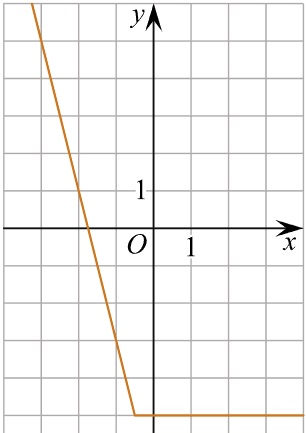
\includegraphics[align=t, width=\textwidth]{pics/G111M4C5-5.jpg}
		\end{minipage}
		\item
		\begin{minipage}[t]{0.43\textwidth}
			На рисунке изображён график функции вида \(f(x)=ax+|bx+c|+d\), где числа \(a, b, c, d\) --- целые. Найдите корень уравнения \(ax+d=0\).
		\end{minipage}
		\begin{minipage}[c]{0.1\textwidth}
			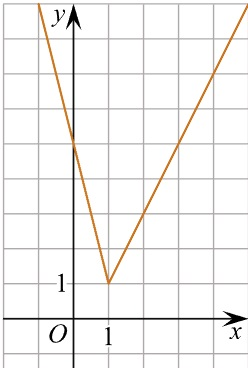
\includegraphics[align=t, width=\textwidth]{pics/G101M4C5-6.jpg}
		\end{minipage}
		\item
		\begin{minipage}[t]{0.43\textwidth}
			На рисунке изображён график функции вида \(f(x)=ax+|bx+c|+d\), где числа \(a, b, c, d\) --- целые. Найдите корень уравнения \(ax+d=19\).
		\end{minipage}
		\begin{minipage}[c]{0.1\textwidth}
			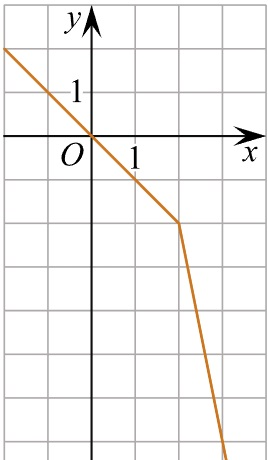
\includegraphics[align=t, width=\textwidth]{pics/G101M4C5-9.jpg}
		\end{minipage}
	\end{listofex}
\end{class}
%
%===============>>  Домашняя работа 3  <<===============
%
%\begin{homework}[number=2]
%	\begin{listofex}
%
%	\end{listofex}
%\end{homework}
%\newpage
%\title{Подготовка к проверочной работе}
%\begin{listofex}
%	
%\end{listofex}
%
%===============>>  Занятие 6  <<===============
%
\begin{class}[number=6]
	\begin{listofex}
<<<<<<< HEAD
<<<<<<< HEAD
	\item Решить систему неравенств:
	\[ \left\{
	\begin{array}{l}
		5(4x+3)-3(4x+5)\le8x+9,\\
		\dfrac{x+2}{4}+\dfrac{x+4}{2}\ge\dfrac{x+3}{5}+\dfrac{x+5}{3}.
	\end{array}
	\right. \]
	\item Решите двойное неравенство: \( 2x+3\le5x^2-9x+5\le7x+2 \).
	\item Гоночный автомобиль разгоняется на прямолинейном участке шоссе с постоянным ускорением \( a \) км/ч\( ^2 \). Скорость \( v \)  в конце пути вычисляется по формуле \( v=\sqrt{2la} \), где \( l \) – пройденный автомобилем путь в км. Определите ускорение, с которым должен двигаться автомобиль, чтобы, проехав \( 250 \) метров, приобрести скорость \( 60 \)км/ч. Ответ выразите в км/ч\( ^2 \).
	\item
	\begin{minipage}[t]{\bodywidth}
		На рисунке изображён график функции \(f(x)=kx+b\). Найдите \(f(-9)\).
	\end{minipage}
	\hspace{0.02\linewidth}
	\begin{minipage}[t]{\picwidth}
		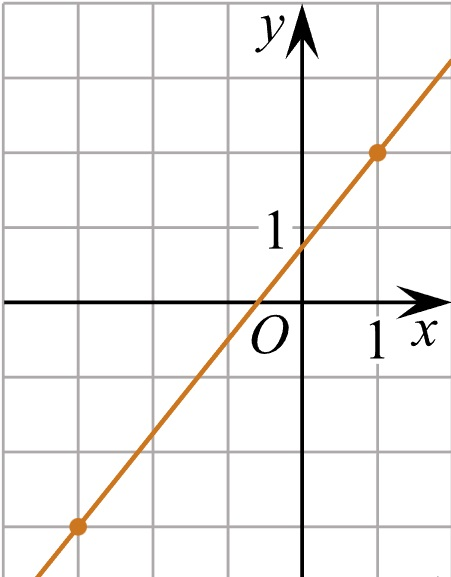
\includegraphics[align=t, width=\textwidth]{pics/G101M4C4-1.jpg}
	\end{minipage}
	\item
	\begin{minipage}[t]{\bodywidth}
		На рисунке изображён график функции вида \(f(x)=ax^2+bx+c\), где числа \(a, b, c\) --- целые. Найдите значение \(f\left( -\mfrac{1}{1}{2} \right)\).
	\end{minipage}
	\hspace{0.02\linewidth}
	\begin{minipage}[t]{\picwidth}
		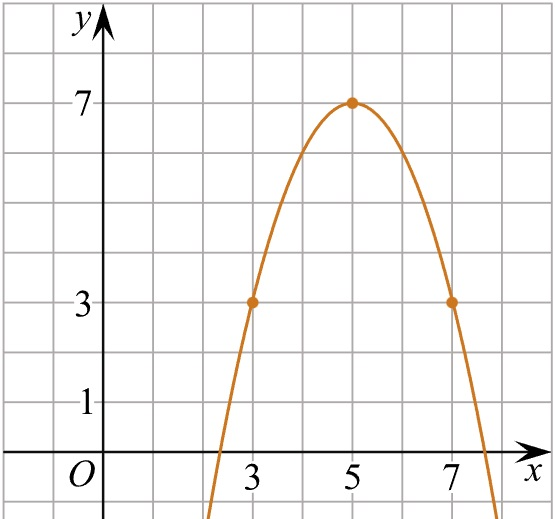
\includegraphics[align=t, width=\linewidth]{pics/G101M4H2-5.jpg}
	\end{minipage}
	\item
	\begin{minipage}[t]{\bodywidth}
		На рисунке изображён график функции вида \[ f(x)=ax+|bx+c|+d, \] где числа \(a, b, c, d\) --- целые. Найдите корень уравнения \(ax+d=-15\).
	\end{minipage}
	\hspace{0.02\linewidth}
	\begin{minipage}[t]{\picwidth}
		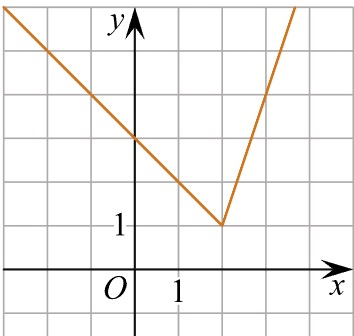
\includegraphics[align=t, width=\linewidth]{pics/G101M4C5-7.jpg}
	\end{minipage}
	\item
	\begin{minipage}[t]{\bodywidth}
		На рисунке изображён график функции вида \[ f(x)=ax+|bx+c|+d, \] где числа \(a, b, c, d\) --- целые. Найдите корень уравнения \(bx+c=2\).
	\end{minipage}
	\hspace{0.02\linewidth}
	\begin{minipage}[t]{\picwidth}
		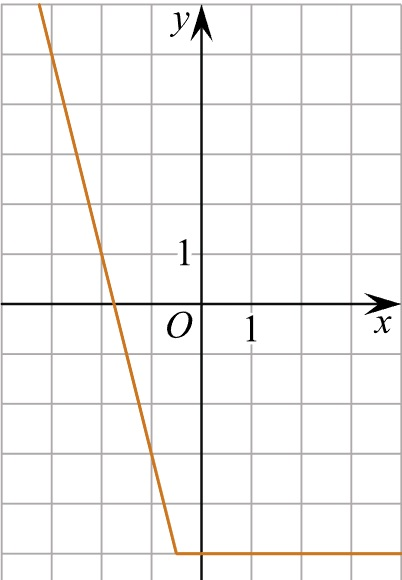
\includegraphics[align=t, width=\linewidth]{pics/G101M4H2-6.jpg}
	\end{minipage}
	\item
	\begin{minipage}[t]{\bodywidth}
		На рисунке изображён график функции вида \[ f(x)=ax-|bx+c|+d, \] где числа \(a, b, c, d\) --- целые. Найдите корень уравнения \(ax+d=-2\).
	\end{minipage}
	\hspace{0.02\linewidth}
	\begin{minipage}[t]{\picwidth}
		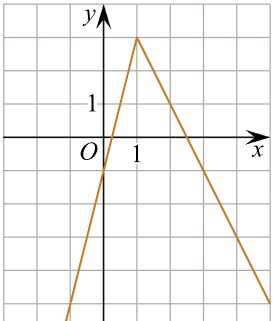
\includegraphics[align=t, width=\linewidth]{pics/G101M4C6-8.jpg}
	\end{minipage}
	\item
	\begin{minipage}[t]{\bodywidth}
		На рисунке изображён график функции вида \[ f(x)=\dfrac{a}{x+b}+c, \] где числа \(a, b, c\) --- целые. Найдите значение \(x\), при котором \(f(x)=-5\).
	\end{minipage}
	\hspace{0.02\linewidth}
	\begin{minipage}[t]{\picwidth}
		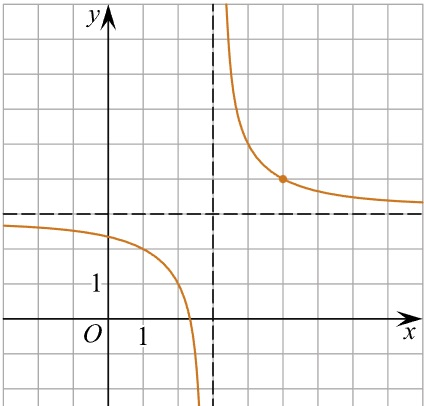
\includegraphics[align=t, width=\linewidth]{pics/G101M4C6-2.jpg}
	\end{minipage}
	\item
	\begin{minipage}[t]{\bodywidth}
		На рисунке изображён график функции вида \[ f(x)=\dfrac{ax+b}{x+c}, \] где числа \(a, b, c\) --- целые. Найдите \(b\).
	\end{minipage}
	\hspace{0.02\linewidth}
	\begin{minipage}[t]{\picwidth}
		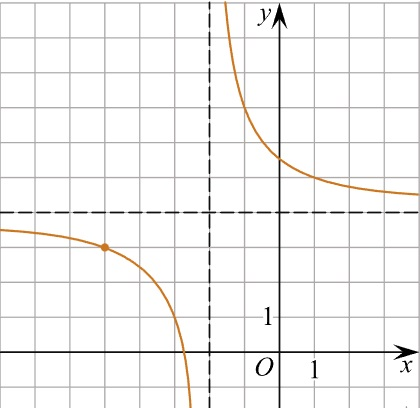
\includegraphics[align=t, width=\linewidth]{pics/G101M4C6-5.jpg}
	\end{minipage}
\end{listofex}
=======
=======
>>>>>>> b62000d7fbf6a0891bc1e1a83262b30711599274
		\item
		\begin{minipage}[t]{0.43\textwidth}
			На рисунке изображён график функции вида \(f(x)=ax+|bx+c|+d\), где числа \(a, b, c, d\) --- целые. Найдите корень уравнения \(ax+d=-15\).
		\end{minipage}
		\begin{minipage}[c]{0.1\textwidth}
			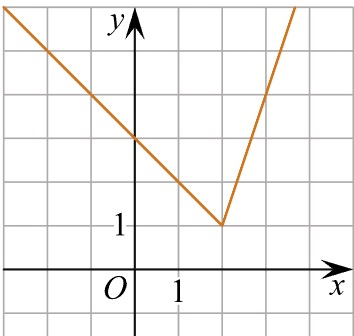
\includegraphics[align=t, width=\textwidth]{pics/G101M4C5-7.jpg}
		\end{minipage}
		\item
		\begin{minipage}[t]{0.43\textwidth}
			На рисунке изображён график функции вида \(f(x)=ax-|bx+c|+d\), где числа \(a, b, c, d\) --- целые. Найдите корень уравнения \(ax+d=-2\).
		\end{minipage}
		\begin{minipage}[c]{0.1\textwidth}
			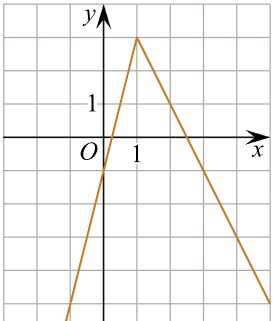
\includegraphics[align=t, width=\textwidth]{pics/G101M4C6-8.jpg}
		\end{minipage}
		\item
		\begin{minipage}[t]{0.43\textwidth}
			На рисунке изображён график функции вида \(f(x)=ax-|bx+c|+d\), где числа \(a, b, c, d\) --- целые. Найдите корень уравнения \(ax=d\).
		\end{minipage}
		\begin{minipage}[c]{0.1\textwidth}
			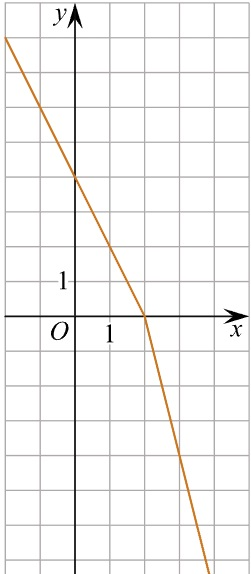
\includegraphics[align=t, width=\textwidth]{pics/G111M4C6-1.jpg}
		\end{minipage}
		\item
		\begin{minipage}[t]{0.43\textwidth}
			На рисунке изображён график функции вида \(f(x)=ax-|bx+c|+d\), где числа \(a, b, c, d\) --- целые. Найдите корень уравнения \(ax+d=0\).
		\end{minipage}
		\begin{minipage}[c]{0.1\textwidth}
			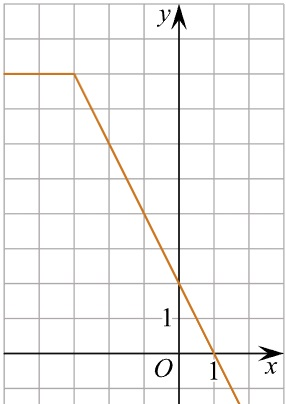
\includegraphics[align=t, width=\textwidth]{pics/G111M4C6-2.jpg}
		\end{minipage}
		\item
		\begin{minipage}[t]{0.43\textwidth}
			На рисунке изображён график функции вида \(f(x)=ax+|bx+c|+d\), где числа \(a, b, c, d\) --- целые. Найдите корень уравнения \(ax+d=0\).
		\end{minipage}
		\begin{minipage}[c]{0.1\textwidth}
			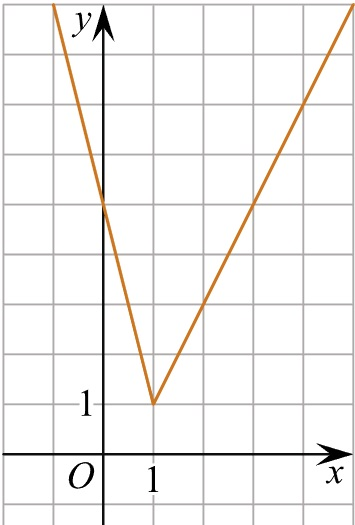
\includegraphics[align=t, width=\textwidth]{pics/G111M4C6-3.jpg}
		\end{minipage}
		\item
		\begin{minipage}[t]{0.43\textwidth}
			На рисунке изображён график функции вида \(f(x)=\dfrac{a}{x+b}+c\), где числа \(a, b, c\) --- целые. Найдите значение \(x\), при котором \(f(x)=-5\).
		\end{minipage}
		\begin{minipage}[c]{0.1\textwidth}
			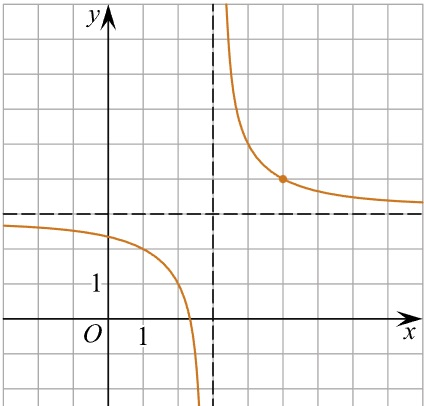
\includegraphics[align=t, width=\textwidth]{pics/G101M4C6-2.jpg}
		\end{minipage}
		\item
		\begin{minipage}[t]{0.43\textwidth}
			На рисунке изображён график функции вида \(f(x)=\dfrac{a}{x+b}+c\), где числа \(a, b, c\) --- целые. Найдите значение \(x\), при котором \(f(x)=2,5\).
		\end{minipage}
		\begin{minipage}[c]{0.1\textwidth}
			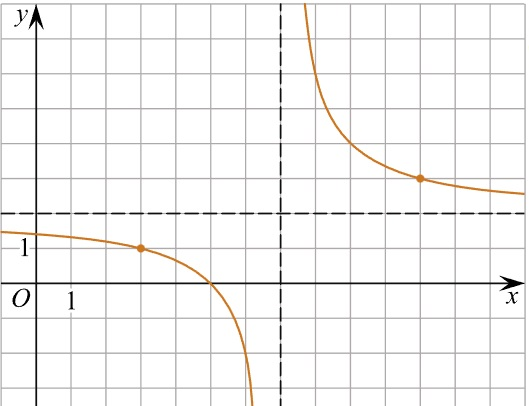
\includegraphics[align=t, width=\textwidth]{pics/G101M4C6-3.jpg}
		\end{minipage}
		\item
		\begin{minipage}[t]{0.43\textwidth}
			На рисунке изображён график функции вида \(f(x)=\dfrac{a}{x+b}+c\), где числа \(a, b, c\) --- целые. Найдите значение \(x\), при котором \(f(x)=-1,125\).
		\end{minipage}
		\begin{minipage}[c]{0.1\textwidth}
			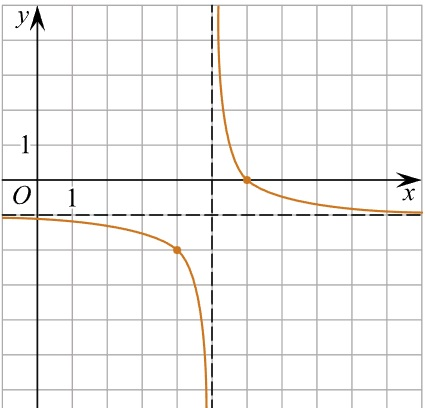
\includegraphics[align=t, width=\textwidth]{pics/G101M4C6-4.jpg}
		\end{minipage}
		\item
		\begin{minipage}[t]{0.43\textwidth}
			На рисунке изображён график функции вида \(f(x)=\dfrac{ax+b}{x+c}\), где числа \(a, b, c\) --- целые. Найдите \(b\).
		\end{minipage}
		\begin{minipage}[c]{0.1\textwidth}
			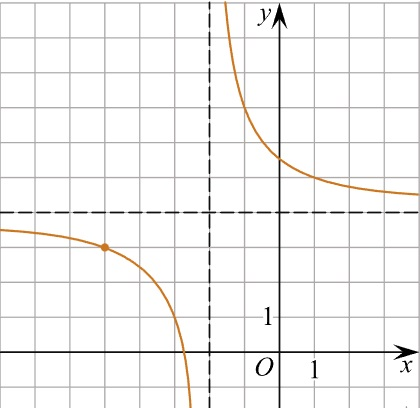
\includegraphics[align=t, width=\textwidth]{pics/G101M4C6-5.jpg}
		\end{minipage}
		\item
		\begin{minipage}[t]{0.43\textwidth}
			На рисунке изображён график функции вида \(f(x)=\dfrac{ax+b}{x+c}\), где числа \(a, b, c\) --- целые. Найдите \(b\).
		\end{minipage}
		\begin{minipage}[c]{0.1\textwidth}
			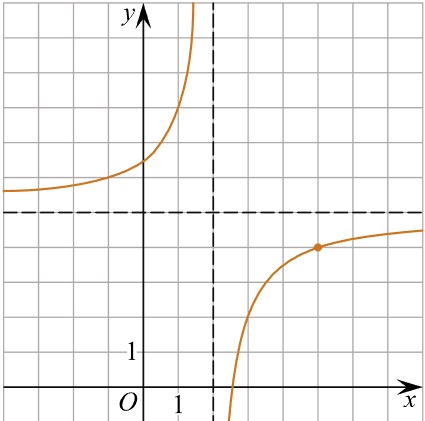
\includegraphics[align=t, width=\textwidth]{pics/G101M4C6-6.jpg}
		\end{minipage}
		\item
		\begin{minipage}[t]{0.43\textwidth}
			На рисунке изображён график функции вида \(f(x)=\dfrac{ax+b}{x+c}\), где числа \(a, b, c\) --- целые. Найдите \(b\).
		\end{minipage}
		\begin{minipage}[c]{0.1\textwidth}
			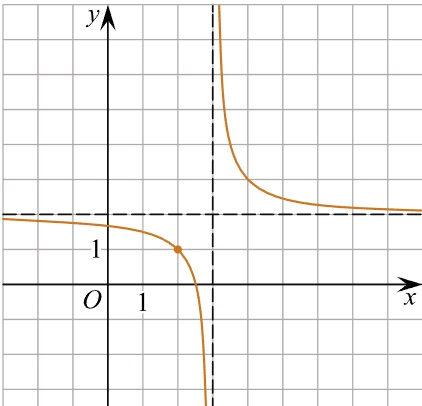
\includegraphics[align=t, width=\textwidth]{pics/G101M4C6-7.jpg}
		\end{minipage}
	\end{listofex}
<<<<<<< HEAD
>>>>>>> 1b9278f8ffbcfbf3d0e771c55020f1e26dc94853
=======
	\item Решить систему неравенств:
	\[ \left\{
	\begin{array}{l}
		5(4x+3)-3(4x+5)\le8x+9,\\
		\dfrac{x+2}{4}+\dfrac{x+4}{2}\ge\dfrac{x+3}{5}+\dfrac{x+5}{3}.
	\end{array}
	\right. \]
	\item Решите двойное неравенство: \( 2x+3\le5x^2-9x+5\le7x+2 \).
	\item Гоночный автомобиль разгоняется на прямолинейном участке шоссе с постоянным ускорением \( a \) км/ч\( ^2 \). Скорость \( v \)  в конце пути вычисляется по формуле \( v=\sqrt{2la} \), где \( l \) – пройденный автомобилем путь в км. Определите ускорение, с которым должен двигаться автомобиль, чтобы, проехав \( 250 \) метров, приобрести скорость \( 60 \)км/ч. Ответ выразите в км/ч\( ^2 \).
	\item
	\begin{minipage}[t]{\bodywidth}
		На рисунке изображён график функции \(f(x)=kx+b\). Найдите \(f(-9)\).
	\end{minipage}
	\hspace{0.02\linewidth}
	\begin{minipage}[t]{\picwidth}
		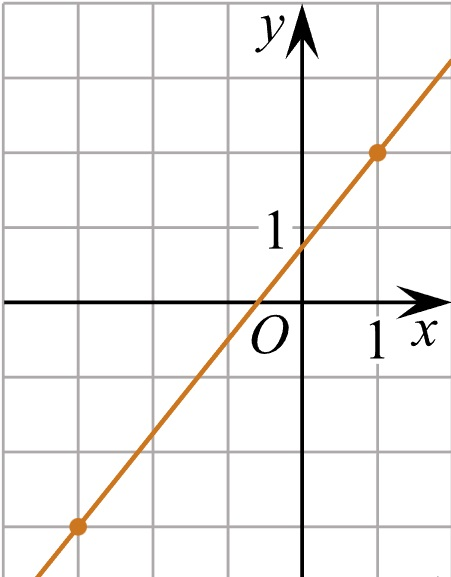
\includegraphics[align=t, width=\textwidth]{pics/G101M4C4-1.jpg}
	\end{minipage}
	\item
	\begin{minipage}[t]{\bodywidth}
		На рисунке изображён график функции вида \(f(x)=ax^2+bx+c\), где числа \(a, b, c\) --- целые. Найдите значение \(f\left( -\mfrac{1}{1}{2} \right)\).
	\end{minipage}
	\hspace{0.02\linewidth}
	\begin{minipage}[t]{\picwidth}
		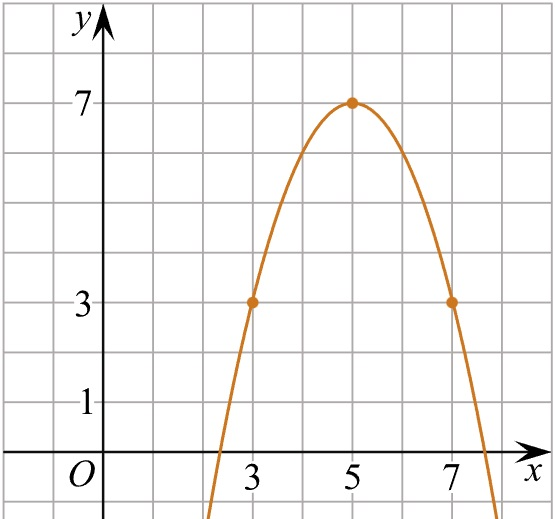
\includegraphics[align=t, width=\linewidth]{pics/G101M4H2-5.jpg}
	\end{minipage}
	\item
	\begin{minipage}[t]{\bodywidth}
		На рисунке изображён график функции вида \[ f(x)=ax+|bx+c|+d, \] где числа \(a, b, c, d\) --- целые. Найдите корень уравнения \(ax+d=-15\).
	\end{minipage}
	\hspace{0.02\linewidth}
	\begin{minipage}[t]{\picwidth}
		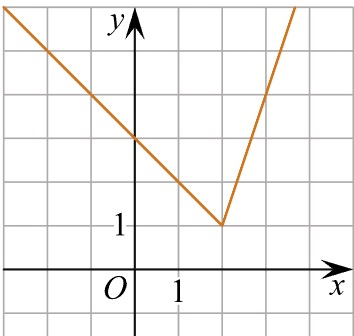
\includegraphics[align=t, width=\linewidth]{pics/G101M4C5-7.jpg}
	\end{minipage}
	\item
	\begin{minipage}[t]{\bodywidth}
		На рисунке изображён график функции вида \[ f(x)=ax+|bx+c|+d, \] где числа \(a, b, c, d\) --- целые. Найдите корень уравнения \(bx+c=2\).
	\end{minipage}
	\hspace{0.02\linewidth}
	\begin{minipage}[t]{\picwidth}
		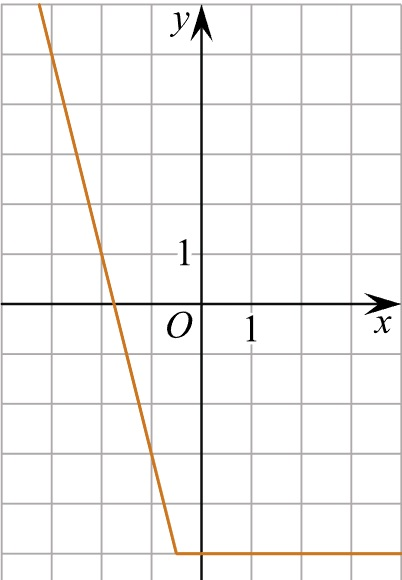
\includegraphics[align=t, width=\linewidth]{pics/G101M4H2-6.jpg}
	\end{minipage}
	\item
	\begin{minipage}[t]{\bodywidth}
		На рисунке изображён график функции вида \[ f(x)=ax-|bx+c|+d, \] где числа \(a, b, c, d\) --- целые. Найдите корень уравнения \(ax+d=-2\).
	\end{minipage}
	\hspace{0.02\linewidth}
	\begin{minipage}[t]{\picwidth}
		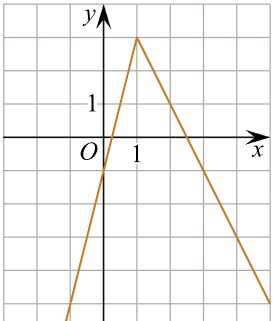
\includegraphics[align=t, width=\linewidth]{pics/G101M4C6-8.jpg}
	\end{minipage}
	\item
	\begin{minipage}[t]{\bodywidth}
		На рисунке изображён график функции вида \[ f(x)=\dfrac{a}{x+b}+c, \] где числа \(a, b, c\) --- целые. Найдите значение \(x\), при котором \(f(x)=-5\).
	\end{minipage}
	\hspace{0.02\linewidth}
	\begin{minipage}[t]{\picwidth}
		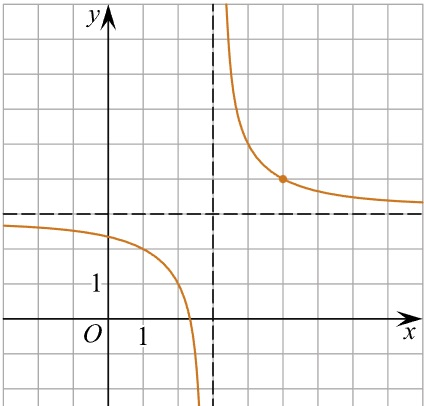
\includegraphics[align=t, width=\linewidth]{pics/G101M4C6-2.jpg}
	\end{minipage}
	\item
	\begin{minipage}[t]{\bodywidth}
		На рисунке изображён график функции вида \[ f(x)=\dfrac{ax+b}{x+c}, \] где числа \(a, b, c\) --- целые. Найдите \(b\).
	\end{minipage}
	\hspace{0.02\linewidth}
	\begin{minipage}[t]{\picwidth}
		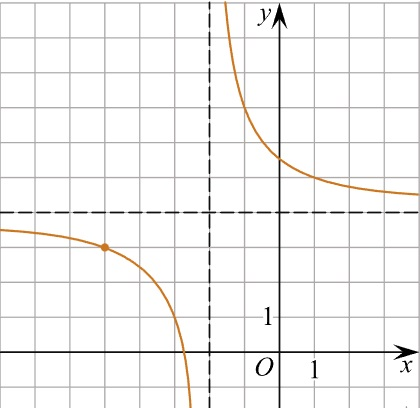
\includegraphics[align=t, width=\linewidth]{pics/G101M4C6-5.jpg}
	\end{minipage}
\end{listofex}
>>>>>>> b62000d7fbf6a0891bc1e1a83262b30711599274
\end{class}
%
%===============>>  Провечная работа  <<===============
%
%\begin{exam}
%	\begin{listofex}
%	
%	\end{listofex}
%\end{exam}